Wir konnten fast all unsere Anforderungen erfüllen.

\section{KZO}
% \includegraphics[height=18cm]{resources/diagrams/use-case}
\begin{enumerate}
    \item \textbf{Zeit} \\
        Geplant war ungefähr eine Lektion pro Woche. Wir haben die geschätzten 50 Stunden um einen Faktor von sechs überschritten. Unser gemessener Zeitaufwand, während aktivem Programmieren,
        beträgt über 330 Stunden. Da sind die Stunden, in denen wir uns in der Freizeit, und mit Herrn Hunziker getroffen haben, gar nicht notiert.
    \item \textbf{Begleitperson} \\
        Wir hatten zum Glück kein Problem eine Begleitperson zu finden. Martin Hunziker war gerne bereit unsere Arbeit im Blick zu behalten.
    \item \textbf{Plagiat} \\
        Zwar sind einige Grafiken aus dem Internet, jedoch sind alle Nutzungsfrei. Auch sonst haben wir keinen Code geklaut und verwendet. 
\end{enumerate}

\subsection*{Notwendig}
\begin{itemize}
    \item \textbf{System} \\
        Unser Spiel funktioniert sowohl auf macOS als auch auf Windows. Dies ausserdem mit einer FPS von 300, bis teilweise 500, bei den meisten modernen Geräten
    \item \textbf{Benutzeroberfläche} \\
    \begin {itemize}
        \item \textbf{Startpage} \\
        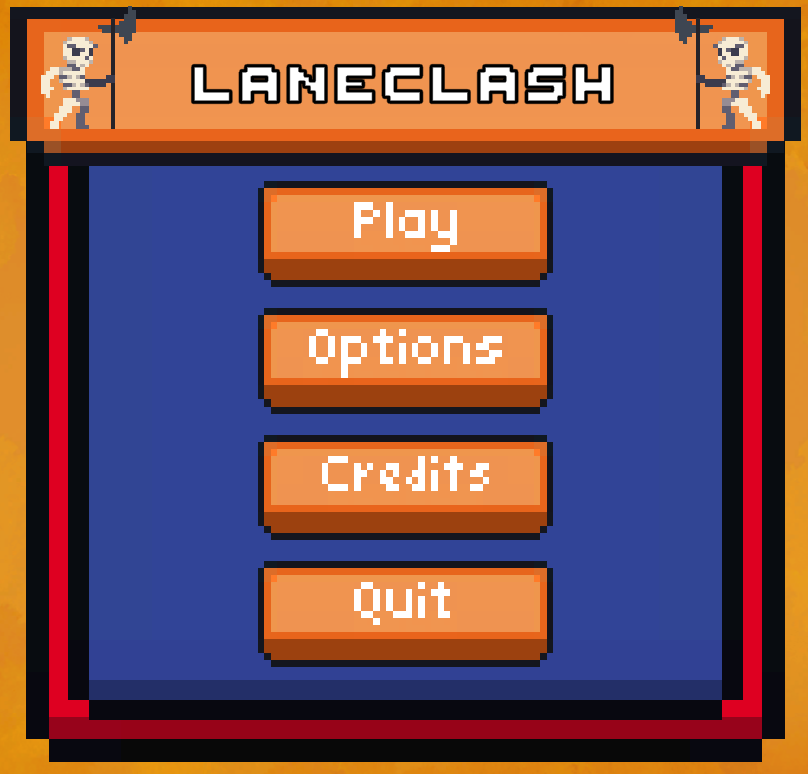
\includegraphics[height=7cm]{resources/laneclash.png}\\
        Unsere Startseite hat einen ''Spielen''-Knopf, einen ''Einstellungen''-Knopf, einen ''Credits''-Knopf und einen ''Verlassen''-Knopf. Unsere vereinzelnten Tester bewerteten die Startseite
        als intuitiv verständlich. Bedienbar mit der Maus, hatten die Tester keine Probleme sich zurechtzufinden.
    \end {itemize}

    \item \textbf{Lokaler Multiplayer} \\
        Das Spiel soll im lokalen Netz gespielt werden können. So zum Beispiel mit Freunden oder Familie.
        Es sollte mithilfe der IP-Adresse innerhalb des gleichen Netzes zusammengespielt werden können.
    \item \textbf{Einstellungen} \\
        Auflösung, Vollbild und Lautstärke müssen eingestellt werden können.
    \item \textbf{Kamera} \\
        Die Kamera ist beweglich und das ganze Schlachtfeld ist sichtbar.
    \item \textbf{Truppen} \\
        Es braucht Truppen, die für einen kämpfen können. Diese sind notwendig für den Verlauf des Spieles
        und ohne sie hat das Spiel keinen Sinn.
    \item \textbf{Gewinnmöglichkeit} \\
        Eine Chance das Spiel zu gewinnen oder verlieren und es somit zu beenden. Dies kann sehr simpel
        mit einer Linie vollendet werden, welche beim Überschreiten das Spiel beendet.
    \item \textbf{Lanes} \\
        Unser Spiel ist zwar 2.5D, aber hat dennoch eine Tiefe.
    \item \textbf{Synchronisation} \\
        Unser Spiel soll in Echtzeit spielbar sein, deswegen müssen die beiden Spieler Synchronisiert das Gleiche sehen. Eine De-Synchronisation wäre verheerend. 
    \item \textbf{Crossplay}
        Die Möglichkeit sich mit einem Windows Rechner und einem macOS Rechner zu verbinden und zusammenzuspielen.
\end{itemize}

\subsection*{Anvisiert}
\begin{itemize}
    \item \textbf{Helden} \\
        Beide Spieler haben eine Art Truppe, welche ihre Siegeslinie beschützt. Sie haben einen Racheeffekt, welcher die
        Lane ausradiert, damit das Spiel nicht sofort vorbei ist.
    \item \textbf{Design} \\
        Das Spiel sollte vom Aussehen her was hergeben. Es sollte nicht wie ein Prototyp, sondern wie ein 
        vollendetes Spiel aussehen. 
    \item \textbf{Deck} \\
        Zu Beginn Spieler könne ihr eigenes Deck aus einer Auswahl von Karten zusammenstellen. Im Spiel werden davon per Zufall Karten gezogen.
    \item \textbf{Bot} \\
        Ein sehr simpler Algorithmus um alleine gegen den Computer zu spielen auf den Schwierigkeitsstufen \textit{'Einfach', 'Mittel', 'Schwierig'}.
        Es sollen rein zufällig Truppen geschickt werden, bei höherer Schwierigkeit mehr.
    \item \textbf{Truppen}
    \begin{itemize}
        \item \textbf{Nahkampf}
            Eine Truppe mit wenig Reichweite.
        \item \textbf{Fernkampf}
            Eine Truppe die auf Reichweite angreift. Sie scheisst Projektive, zum Beispiel ein Bogenschütze,
            der mit Pfeilen schiesst.
        \item \textbf{Suizid}
            Eine Truppe die bei Berührung mit einem Gegner stirbt und einen Effekt auslöst.
    \end{itemize}
    \item \textbf{Effekte}
    \begin{itemize}
        \item \textbf{Gift:}
            Zeitlich limitierter und wiederholender Schadenseffekt. Eine visuelle Markierung soll vorhanden sein
            und das gleiche Gift, also der gleichen Truppe, soll nur einmal auf jemanden sein.
        \item \textbf{Dorn:}
            Truppen, welche Charaktere mit Dorn attackieren, erhalten schaden. Soll nach Auswahl auf Nahkämpfer,
            Fernkämpfer oder beides wirken.
        \item \textbf{Rache:}
            Truppen mit Rache haben einen Effekt nach ihrem Tod. Zum Beispiel eine Truppe beschwören oder Schaden verursachen.
    \end{itemize}
\end{itemize}

\subsection*{Möglichkeiten}
\begin{itemize}
    \item \textbf{Zauber} \\
        Als Alternative sollen nicht alle Karten einfach eine Truppe herbeirufen. Gewisse Karten sollten nur einen Effekt auslösen.
        Beispiele für Zauber:
            "Heile deine Helden um 5 leben"
            "Gib deinen Helden 5 Rüstung"
            "Verursache allen gegnerischen Truppen 5 Schaden"
            "Ziehe 3 Karten"
    \item \textbf{Monetarisierung} \\
    Hierfür sind uns drei Möglichkeiten eingefallen, hier jeweils die Vor- und Nachteile:
    \begin{enumerate}
        \item \textbf{Kaufbare Gegenstände}
        \begin{itemize}
            \item[+] Vielseitige und Nachhaltige Monetarisierung. Neue Features, bedeuten auch neue Geldmöglichkeit. Die Inhalte sollten
                     auch erspielbar sein, somit kann bezahlen zwar zu Vorteilen führen, jedoch mit viel Spielen trotzdem erreichbar sein.
            \item[-] Pay-to-Win
        \end{itemize}
        \item \textbf{Skins}
        \begin{itemize}
            \item[+] Weit verbreitet und sehr beliebt bei Spielern. Gibt keinem Spieler Vorteile
            \item[-] Wenig Nutzen und sehr aufwändig. Neue Designs zu erstellen, wäre bei uns nicht so sinnvoll.
                     Wir haben noch sehr viel Features zu implementieren und sind nicht Designer. Für uns braucht es sehr
                     viel Zeit eine brauchbare Darstellung zu erstellen und der Mehrwert, welcher dem Spiel beigetragen wird, ist marginal.
        \end{itemize}
        \item \textbf{Kostenpflichtiges Spiel}
        \begin{itemize}
            \item[+] Einmalige Bezahlung, was für viele Nutzer lukrativer ist. Jedoch gilt dies vor allem bei Singleplayer Spielen.
            \item[-] Wir nehmen an, dass wenige Leute bereit wären, Geld für unser Spiel zu bezahlen.
                    Dafür wird es nicht genug ausgereift sein.
                    Auch ist diese Methodik nicht nachhaltig und führt nur zu einer einmaligen Geldspritze.
                    Viele grössere Spiele führen deshalb später
                    DLCs ein, um das Spiel zu erweitern.
                    Jedoch ist dies bei einem Multiplayer Spiel Pay-to-Win.
                    Abschliessen müssten wir höchstwahrscheinlich selbst Geld vorauswerfen, um unser Spiel anbieten zu können, z.B. auf Steam.
        \end{itemize}
        
    \end{enumerate}
    \item \textbf{Helden} \\
        Eine Auswahl von Helden, mit unterschiedlichem Schaden, Leben und Effekten, würde das Spiel nochmals spannender machen. Auch sollten gewisse Truppen auf bestimmte Helden limitiert sein. 
    \item \textbf{Design} \\
        Wenn die Zeit vorhanden ist, kann das Design immer verbessert werden. Hier gehts es aber um den Feinschliff, z.B. mehr Hintergründe, und mehr Dinge selbst zu designen.
    \item \textbf{Tutorial} \\
        Eine Anleitung für Anfänger wäre sehr schön. Sie soll neuen Spielern das Anfangen erleichtern. Es sollte aber auch überspringbar sein,
        damit alte Spieler, es nicht nochmals spielen müssen. Es soll nicht lange sein und nicht schwierig. Dennoch soll es alle Mechaniken des Spiels
        erklären, am besten Anhand von Gameplay.
    \item \textbf{Truppen}
        Weitere Truppen können jederzeit erstellt werden. Hier ist kein Limit gesetzt. Leben, Schaden, Darstellung, Effekt und vieles mehr kann angepasst werden.
    \item Effekte
    \begin{itemize}
        \item \textbf{Wiederbelebung:}
            Die Truppe wird wiederbelebt, sofort an Ort und Stelle oder mit einer Verzögerung am Startpunkt.
        \item \textbf{Rüstung:}
            Die Truppe hat zusätzlichen zu den Leben auch Rüstung. Die Rüstung wird zuerst abgezogen und hat im Gegensatz zum Leben keine Limite.
        \item \textbf{Aura:}
            Die Truppe fügt gegnerischen Truppen in einem gewissen Radius permanent Schaden zu.
    \end{itemize}
    \item \textbf{Mehrsprachig} \\
        Das Spiel soll in Englisch, Deutsch und Französisch spielbar sein.
\end{itemize}

\subsection*{Verworfen}
\begin{itemize}
    \item \textbf{Online Multiplayer} \\
        Besser als ein Multiplayer, der limitiert auf dasselbe Netz ist, ist ein Multiplayer, der weltweit verfügbar ist. Jedoch ist von einem Computer auf einen anderen zu
        verbinden dank der Firewall von Router und Computer, nahezu unmöglich. Es würden sich viele weitere Probleme ergeben, wie zum Beispiel Port-Forwarding. Dies ist einer der Gründe, weshalb ein Server sehr praktisch ist. Mit diesem ist dieses
        Problem gelöst. Server sind aber teuer und aufwändig. Wir müssten allerdings das ganze Multiplayer System unseres Spieles anpassen, was einen kompletten Recode zur Folge hätte.
    \item \textbf{Shop} \\
        Nicht alle Karten sind von Beginn an freigeben, sondern müssen freigespielt werden.
        So kann zum Beispiel eine Ingame Währung erspielt werden und damit im Shop Karten oder sonstige Dinge gekauft werden.
        Der Shop kann mit Zahlungsmethoden ausgestattet werden und so zur Monetarisierung beitragen.
        Jedoch ist ein Shop ohne Anti-Cheat und/oder Server die perfekte Angriffsfläche für Cheater und hat somit nicht viel Sinn.
    \item \textbf{Kampagne} \\
        Singleplayer gegen bestimmte vorprogrammierte Gegner. Sie sollen immer schwieriger werden und bestimmte Herausforderungen mit sich bringen.
        Bei Vollendung werden Belohnungen verteilt.
    \item \textbf{Anti-Cheat} \\
        Dies ist für uns ohne Erfahrung in diesem Bereich und einem lokal berechnetet Spiel ein Ding der Unmöglichkeit.
        Wir haben keine Erfahrung in diesem Bereich und es ist ein extrem komplexes Thema.
    \item \textbf{Errungenschaften} \\
        Eine Übersicht und die Möglichkeit die Errungenschaften zu erfüllen.
        Gegebenenfalls Belohnungen verteilen, wie zum Beispiel bestimmte Karten freischalten.
        Diese Erweiterung ist keines Falls notwendig und ein absolutes nice-to-have Feature.
\end{itemize}